\documentclass[14pt]{beamer}
\usepackage[utf8]{inputenc}
\usepackage[T1]{fontenc}
\usepackage{lmodern}
\usepackage[english]{babel}
\usepackage{amsmath}
\usepackage{amsfonts}
\usepackage{amssymb}
\usepackage{graphicx}
\usetheme{default}
\begin{document}
	\addtocounter{framenumber}{-1}
	
	\author{Sewade Ogun}
	\title{Adversarial Examples}
	\subtitle{A new evil in town to be aware of...}
	%\logo{}
	\institute{AMMI, AIMS}
	\date{Ghana, \today}
	%\subject{}
	%\setbeamercovered{transparent}
	%\setbeamertemplate{navigation symbols}{}
	\begin{frame}[plain]
	\maketitle
	\begin{figure}
		\centering
		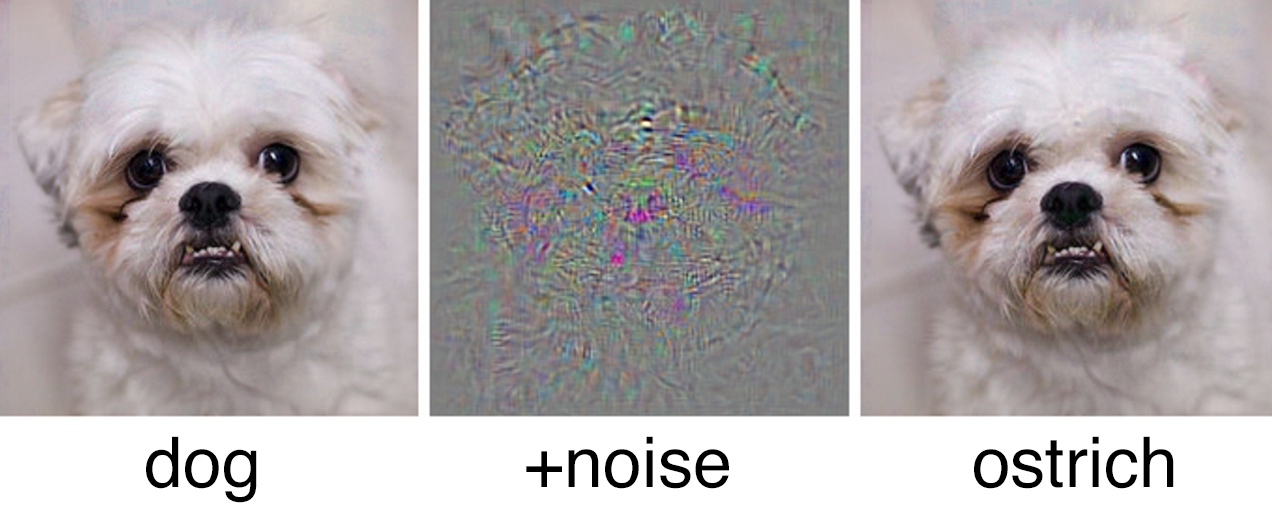
\includegraphics[width=0.7\linewidth]{img/dog}
		\label{fig:dog}
	\end{figure}
\end{frame}

\section{Objectives}
\begin{frame}
\frametitle{Objectives}
\begin{enumerate}
	\item To show the effect and effectiveness of adversarial examples in machine learning predictions
	\item To understand the adversary, and determine how to combat them
	\item To enlighten the audience on adversarial security measures.
\end{enumerate}

\end{frame}

\begin{frame}
	\frametitle{Outlines}
	\tableofcontents
\end{frame}

\section{Introduction}
\begin{frame}
\frametitle{Introduction}
	\begin{itemize}
		\item[o] An \textbf{adversarial example} is an instance with small, intentional feature perturbations that cause a machine learning model to make a false prediction.\protect\footnotemark
		\footnotetext{https://christophm.github.io/interpretable-ml-book/adversarial.html}
		
		\item[o] Adversarial examples are a type of \textbf{counterfactual examples} with the aim to deceive the model, not interpret it.
		
		\begin{figure}
			\centering
			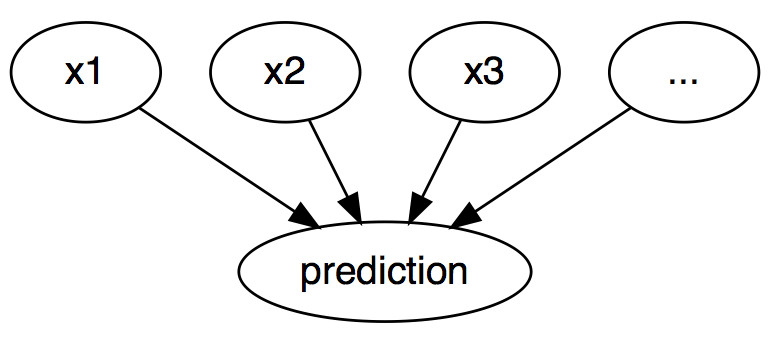
\includegraphics[width=0.7\linewidth]{img/graph}
			\caption{Causal relationships between inputs of a machine learning model and the predictions}
			\label{fig:graph}
		\end{figure}
		
	\end{itemize}
	
\end{frame}

\section{Properties of Counterfactual Instance}
\begin{frame}
\frametitle{Properties of Counterfactual Instance}
\begin{itemize}
	\item[o] A counterfactual should be as \textbf{similar} as possible to the instance regarding feature values
	\item[o] Should change as \textbf{few} features as possible.
	\item[o] A counterfactual instance \textbf{should} have feature values that are likely.
	\item[o] It should produce the predefined prediction as closely as possible.
\end{itemize}
\end{frame}


\section{Examples}
\begin{frame}
\frametitle{Examples}
\begin{enumerate}
	\item You submit your details for an offer in such a way that the machine classify you as eligible.
	\item A spam detector fails to classify an email as spam. The spam mail has been designed to resemble a normal email, but with the intention of cheating the recipient.
	\item A machine-learning powered scanner scans suitcases for weapons at the airport. A knife was developed to avoid detection by making the system think it is an umbrella.
	\item Self-driving cars can be deceived by images to misclassify stop-signs.
\end{enumerate}
\end{frame}

\subsection{Techniques}
\begin{frame}
\frametitle{Techniques}
\begin{enumerate}
	\item Minimize the distance between the adversarial example and the instance to be manipulated, while shifting the prediction to the desired (adversarial) outcome. 
	\item Perturb the example using the gradients of the model, which of course only works with gradient based models such as neural networks,
	\item Use the prediction function to train a model to generate new examples, (which makes these methods model-agnostic.)
\end{enumerate}
Our focus will be on how adversarial examples affect image classifiers with deep neural networks.
\end{frame}

\subsection{Gradient based optimization approach}
\begin{frame}
\frametitle{Gradient based optimization approach}
$$\min loss(f(x + p), y_{adv}) + c.|p|$$
{\small where x is an image, p is the changes to the pixels to create an adversarial image, $y_{adv}$ is the desired outcome class, and the parameter c is a balancing factor.}

\begin{figure}
	\centering
	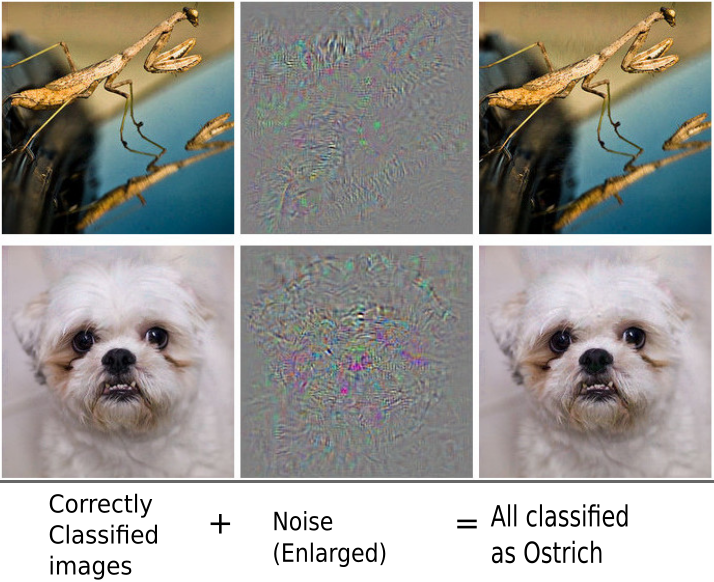
\includegraphics[width=0.35\linewidth, height=0.35\textheight]{img/adv_ex}
	\caption[Examples generated on Alexnet]{Examples generated on Alexnet using GB\protect\footnotemark}
	\label{fig:advex}
\end{figure}
\footnotetext{{\tiny Szegedy, Christian, et al. “Intriguing properties of neural networks.”(2013)}}

\end{frame}

\subsection{Fast gradient sign method}
\begin{frame}
\frametitle{Fast gradient sign method}
$$x_{adv} = x + \epsilon Sign(\nabla_xJ(\theta,x,y))$$
where $x$ is the gradient of the models loss function with respect to the original input pixel vector $x, y$ is the true label vector for $x$ and $\theta$ is the model parameter vector.
\begin{figure}
	\centering
	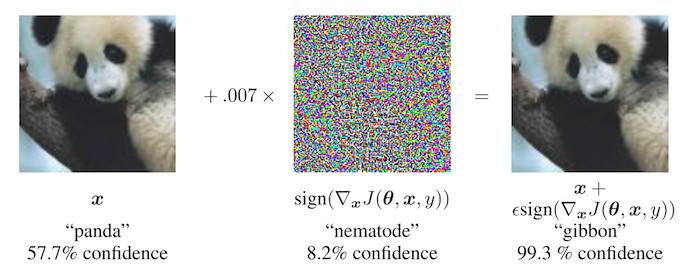
\includegraphics[width=0.7\linewidth, height=0.3\textheight]{img/adversarial-panda}
	\caption{NN predicts Gibbon for a perturbed panda image\protect\footnotemark}
	\label{fig:adversarial-panda}
\end{figure}
\footnotetext{{\tiny Goodfellow et al. “Explaining and harnessing adversarial examples.”(2014)}}
\end{frame}

\subsection{1-pixel attack}
\begin{frame}
\frametitle{Changing a single pixel}
Uses \textbf{differential evolution} to find out which pixel is to be changed and how.
\begin{figure}
	\centering
	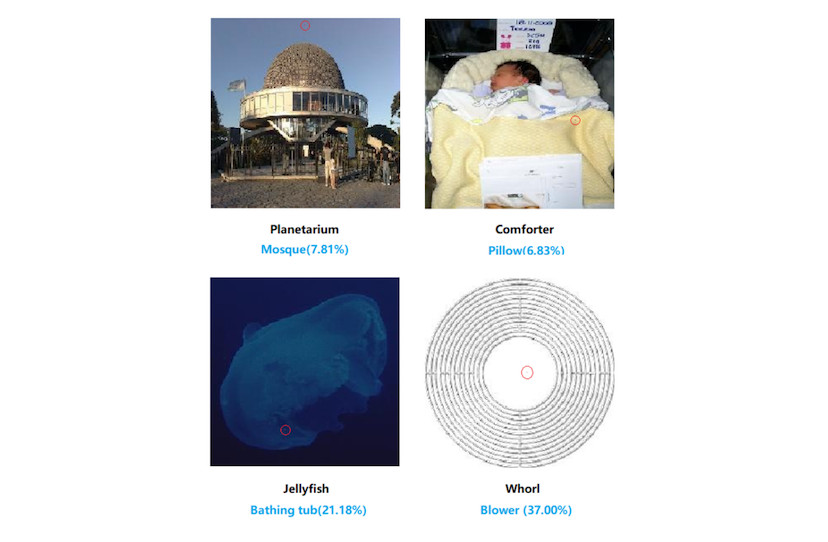
\includegraphics[width=0.8\linewidth]{img/adversarial-1pixel}
	\caption{Changing a single pixel (marked with circles) to deceive a NN to predict the wrong class instead of the original class.\protect\footnotemark}
	\label{fig:adversarial-1pixel}
\end{figure}


\footnotetext{{\tiny Su et al. “One pixel attack for fooling deep neural networks.”(2019).}}
\end{frame}

\end{document}